\clearpage
\section{远处地面的纹理闪动}
\label{sec:texture-minification}
\fancypagestyle{miptexture}{\fancyhead[R]{\sffamily\small\color{Muted}Vulkan / 纹理过滤}}
\thispagestyle{miptexture}

一黑一白的细格铺在地面上。走近能分辨格子，远处一个像素可能盖住几十格，应该看到稳定的灰色。旧版 Vulkan 只上传最大的那张贴图。相机略微向右移动，屏幕像素就会从黑格滑到白格，地面出现了原图中没有的明暗条纹。

\begin{figure}[H]
\centering
\begin{tabular}{@{}ccc@{}}
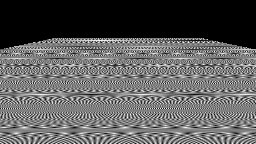
\includegraphics[width=.31\linewidth]{../../../output/profiling/texture-minification/old/frame-b.png} &
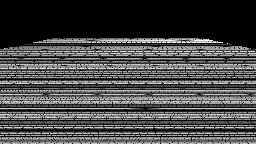
\includegraphics[width=.31\linewidth]{../../../output/profiling/texture-minification/old/motion-x4.png} &

\includegraphics[width=.31\linewidth]{../../../output/profiling/texture-minification/fixed/frame-b.png} \\
{\small 单层贴图} & {\small 旧版两帧的差异} & {\small 修复后的地面}
\end{tabular}
\caption{中图将相机移动前后两张显示图逐像素相减，绝对差放大四倍。地面内部越亮，说明这里闪动越明显。左右图的机位、贴图和曝光一致。}\end{figure}

相机横移 0.007 个场景单位，中央参照点在 $256\times144$ 的画面上只走了 0.206 像素。测试直接读底色，关掉灯光和 TAA，对地面内部相同的 8,256 个像素求两帧线性亮度的平均绝对差。单层贴图读到 $0.09129$；补齐逐级减半的九层贴图后，这组像素的差降到 0。黑白各半的正确亮度是 0.5，第二帧的均值由 0.24262 变为 0.50391。缩图使用 8 位存储，加上纹理单元的采样精度，结果与 0.5 略有距离。

底色图中的字节表达显示用的 sRGB 颜色。显卡在生成缩图、绘制时都先把它们换成线性亮度再过滤。粗糙度等数据直接按数值取平均，透明度也如此。两份 RenderDoc 截帧的地面绘制都在事件 11。黑白格第一次缩小后，底色图灰度字节是 188，数据图是 127。用户把同一张图交给这两种用途时，引擎才各留一份；屏幕上的场景面板仍然只有一层。

RTX 5070 Ti Laptop 的驱动为旧 $256^2$ 贴图要求 262,144 字节显存，新的一条链占 351,232 字节，增加 87 KiB（约 34\%）。此例刻意把一张图同时作底色和材质数据，两条链共 702,464 字节。单用途贴图只付一条链的费用。设置透明阈值 0.5 后，底色的 Alpha 和独立透明图分别用 127 与 128 两个字节验证；左半边均露出背景，拾取为 $-1$，右半边仍是实体 7。

\note{Debug/x64，\path{tests/run_texture_minification.cmd}；两份截帧、原图与显存读数在 \path{output/profiling/texture-minification/}。层级生成见 \path{VulkanDrawResources.cpp} 的 \code{BuildMips}，材质采样见 \path{Platform/Vulkan/Shaders/Mesh.frag}。}
